
%----------------------------------------------------------------------------------------
%	PACKAGES AND DOCUMENT CONFIGURATIONS
%----------------------------------------------------------------------------------------

\documentclass{article}

\usepackage[version=3]{mhchem} % Package for chemical equation typesetting
\usepackage{siunitx} % Provides the \SI{}{} and \si{} command for typesetting SI units
\usepackage{graphicx} % Required for the inclusion of images
\usepackage{natbib} % Required to change bibliography style to APA
\usepackage{amsmath} % Required for some math elements 
\usepackage{amsfonts}
\usepackage{algorithm}
\usepackage{algorithmic}

\setlength\parindent{0pt} % Removes all indentation from paragraphs

\renewcommand{\labelenumi}{\alph{enumi}.} % Make numbering in the enumerate environment by letter rather than number (e.g. section 6)

%\usepackage{times} % Uncomment to use the Times New Roman font

%----------------------------------------------------------------------------------------
%	DOCUMENT INFORMATION
%----------------------------------------------------------------------------------------

\title{A Demo of Reduced Gradient Descent Optimization} % Title

\author{Jiyuan Liu} % Author name

\date{\today} % Date for the report

\begin{document}

\maketitle % Insert the title, author and date

\begin{center}
\begin{tabular}{l r}
Date Performed: & June 13, 2020 \\ % Date the experiment was performed
Partners: & None \\ % Partner names
Supervisor: & Xinwang Liu % Instructor/supervisor
\end{tabular}
\end{center}


\clearpage


% If you wish to include an abstract, uncomment the lines below
% \begin{abstract}
% Abstract text
% \end{abstract}

%----------------------------------------------------------------------------------------
%	SECTION 1
%----------------------------------------------------------------------------------------

\section{Objective}

Defining $\mathbf{M} \in \mathbb{R}^{m\times m}$ a positive-defined symmetric matrix, the optimization problem can be given as 
\begin{equation}\label{eq:obj}
	\begin{split}
		\min_{\boldsymbol{\beta}} \boldsymbol{\beta}^\top\mathbf{M}\boldsymbol{\beta} \quad s.t. \sum_{p=1}^m \beta_p = 1,\; \beta_p\geq 0,\; \forall p.
	\end{split}
\end{equation}

It can be observed that Eq. (\ref{eq:obj}) is convex.
Therefore, the minimum can be found with an unique solution.
In fact, This is a classical Quadratic Programming problem which can be easily solved via \emph{quadprog} function in MATLAB.
But we are going to show how to solve it via Reduced Gradient Descent algorithm. 

%----------------------------------------------------------------------------------------
%	SECTION 2
%----------------------------------------------------------------------------------------

\section{Optimization One}

Directly applying Gradient Descent algorithm is infeasible, for there are constraint on $\boldsymbol{\beta}$.
For ease of expression, The optimization problem is firstly transformed into 
\begin{equation}\label{eq:obj_tran}
	\begin{split}
		\min_{\boldsymbol{\beta}\in \bigtriangleup} &\; \mathcal{J}(\boldsymbol{\beta}) \\
		s.t. & \; \mathcal{J}(\boldsymbol{\beta}) = \boldsymbol{\beta}^\top\mathbf{M}\boldsymbol{\beta},
	\end{split}
\end{equation}
where $\bigtriangleup = \{ \boldsymbol{\beta} \in \mathbb{R}^m\; |\; \sum_{p=1}^m \beta_p = 1,\; \beta_p\geq 0,\; \forall p\}$.
At the same time, $\mathcal{J}(\boldsymbol{\beta})$ is differentiable, and
\begin{equation}\label{eq:obj_derivative}
	\begin{split}
		\frac{\partial \mathcal{J}(\boldsymbol{\beta})}{\partial \boldsymbol{\beta}}\; =\; 2\mathbf{M}\boldsymbol{\beta}
	\end{split}
\end{equation}
To fulfill this goal, we firstly handle the equality constraint by computing the reduced gradient by following \cite{rakotomamonjy2008simplemkl}.
Let $\beta_u$ be a non-zero component of $\boldsymbol{\beta}$ and $\bigtriangledown \mathcal{J}(\boldsymbol{\beta})$ denote the reduced gradient of $\mathcal{J}(\boldsymbol{\beta})$.
The $p$-th ($1\leq p \leq m$) element of $\bigtriangledown \mathcal{J}(\boldsymbol{\beta})$ is
\begin{equation}\label{eq:p_derivative}
	\begin{split}
		[\bigtriangledown \mathcal{J}(\boldsymbol{\beta})]_p = \frac{\partial \mathcal{J}(\boldsymbol{\beta})}{\partial \beta_p} - \frac{\partial \mathcal{J}(\boldsymbol{\beta})}{\partial \beta_u},\; \forall p \neq u
	\end{split}
\end{equation}
and 
\begin{equation}\label{eq:u_derivative}
	\begin{split}
		[\bigtriangledown \mathcal{J}(\boldsymbol{\beta})]_u = \sum_{p=1,p\neq u}^m (\frac{\partial \mathcal{J}(\boldsymbol{\beta})}{\partial \beta_u} - \frac{\partial \mathcal{J}(\boldsymbol{\beta})}{\partial \beta_p}).
	\end{split}
\end{equation}
We choose $u$ to be the index of the largest component of vector $\boldsymbol{\beta}$ which is considered to provide better numerical stability.
The gradients for updating $\boldsymbol{\beta}$ can be given as 
\begin{equation}\label{eq:gradient}
	\begin{split}
		d_p = \left\{
			\begin{array}{ll}
			0	&	\mathrm{if}\; \beta_p=0\; \mathrm{and}\; [\bigtriangledown \mathcal{J}(\boldsymbol{\beta})]_p > 0\\
			- [\bigtriangledown \mathcal{J}(\boldsymbol{\beta})]_p  &  \mathrm{if}\; \beta_p>0\; \mathrm{and}\; p\neq u\\
			- [\bigtriangledown \mathcal{J}(\boldsymbol{\beta})]_u  &  \mathrm{if}\; p=u
			\end{array} \right.
	\end{split}
\end{equation}
This way, $\boldsymbol{\beta}$ can be computed via updating scheme $\boldsymbol{\beta} \leftarrow \boldsymbol{\beta} + \alpha \mathbf{d}$, where $\alpha$ is the step size.
The overall algorithm can be designed in Algorithm \ref{alg:RGD_alg}.


\begin{algorithm}[h]
\caption{A Demo of Reduced Gradient Descent Algorithm}
\label{alg:RGD_alg}
\textbf{Input}: $\mathbf{M}$\\
\textbf{Output}: $\boldsymbol{\beta}$
\begin{algorithmic}[1] %[1] enables line numbers
\STATE initialize $\boldsymbol{\beta}^{(1)}=\mathbf{1}_m/m$, $t=1$ and $flag=1$.
\WHILE{$flag$}
  \STATE compute $\mathbf{d}^{(t)}$ in Eq. (\ref{eq:gradient}).
  \STATE update $\boldsymbol{\beta}^{(t+1)} \leftarrow \boldsymbol{\beta}^{(t)} + \alpha \mathbf{d}^{(t)}$.
  \IF{$\max |\boldsymbol{\beta}^{(t+1)}-\boldsymbol{\beta}^{(t)}| \leq 1e^{-4}$}
  		\STATE $flag$ = 0.
  \ENDIF
  \STATE $t \leftarrow t+1$.
\ENDWHILE
\end{algorithmic}
\end{algorithm}


%----------------------------------------------------------------------------------------
%	SECTION 3
%----------------------------------------------------------------------------------------

\section{Optimization Two}

Directly applying Gradient Descent algorithm is infeasible, for there are constraint on $\boldsymbol{\beta}$.
For ease of expression, The optimization problem is firstly transformed into 
\begin{equation}\label{eq:obj_tran_two}
	\begin{split}
		\min_{\boldsymbol{\beta}\in \bigtriangleup} &\; \mathcal{J}(\boldsymbol{\beta}) \\
		s.t. & \; \mathcal{J}(\boldsymbol{\beta}) = \boldsymbol{\beta}^\top\mathbf{M}\boldsymbol{\beta},
	\end{split}
\end{equation}
where $\bigtriangleup = \{ \boldsymbol{\beta} \in \mathbb{R}^m\; |\; \sum_{p=1}^m \beta_p = 1,\; \beta_p\geq 0,\; \forall p\}$.
At the same time, $\mathcal{J}(\boldsymbol{\beta})$ is differentiable, and
\begin{equation}\label{eq:obj_derivative_two}
	\begin{split}
		\frac{\partial \mathcal{J}(\boldsymbol{\beta})}{\partial \boldsymbol{\beta}}\; =\; 2\mathbf{M}\boldsymbol{\beta}
	\end{split}
\end{equation}
To ensure the constraint $\beta_p \geq 0,\; \forall p$, we compute the derivatives of $\mathcal{J}(\boldsymbol{\beta})$ as 
\begin{equation}
	\begin{split}
		\delta_p = \left\{
			\begin{array}{ll}
			0	&	\mathrm{if}\; \beta_p=0\; \mathrm{and}\; \frac{\partial \mathcal{J}(\boldsymbol{\beta})}{\partial \beta_p} > 0\\
			\frac{\partial \mathcal{J}(\boldsymbol{\beta})}{\partial \beta_p}  &  \mathrm{otherwise}
			\end{array} \right.
	\end{split}
\end{equation}
To ensure $\sum_{p=1}^m \beta_p = 1$, we define the reduced gradient of $\mathcal{J}(\boldsymbol{\beta})$ by following \cite{rakotomamonjy2008simplemkl} as 
\begin{equation}\label{eq:p_derivative_two}
	\begin{split}
		[\bigtriangledown \mathcal{J}(\boldsymbol{\beta})]_p = \delta_p - \delta_u,\; \forall p \neq u
	\end{split}
\end{equation}
and 
\begin{equation}\label{eq:u_derivative_two}
	\begin{split}
		[\bigtriangledown \mathcal{J}(\boldsymbol{\beta})]_u = \sum_{p=1,p\neq u}^m (\delta_u - \delta_p).
	\end{split}
\end{equation}

We choose $u$ to be the index of the largest component of vector $\boldsymbol{\beta}$ which is considered to provide better numerical stability.
The gradients for updating $\boldsymbol{\beta}$ can be obtained as 
\begin{equation}\label{eq:gradient_two}
	\begin{split}
		d_p = - [\bigtriangledown \mathcal{J}(\boldsymbol{\beta})]_p,\; \forall p.
	\end{split}
\end{equation}


This way, $\boldsymbol{\beta}$ can be computed via updating scheme $\boldsymbol{\beta} \leftarrow \boldsymbol{\beta} + \alpha \mathbf{d}$, where $\alpha$ is the step size.
The overall algorithm can be designed in Algorithm \ref{alg:RGD_alg_two}.


\begin{algorithm}[h]
\caption{A Demo of Reduced Gradient Descent Algorithm}
\label{alg:RGD_alg_two}
\textbf{Input}: $\mathbf{M}$\\
\textbf{Output}: $\boldsymbol{\beta}$
\begin{algorithmic}[1] %[1] enables line numbers
\STATE initialize $\boldsymbol{\beta}^{(1)}=\mathbf{1}_m/m$, $t=1$ and $flag=1$.
\WHILE{$flag$}
  \STATE compute $\mathbf{d}^{(t)}$ in Eq. (\ref{eq:gradient_two}).
  \STATE update $\boldsymbol{\beta}^{(t+1)} \leftarrow \boldsymbol{\beta}^{(t)} + \alpha \mathbf{d}^{(t)}$.
  \IF{$\max |\boldsymbol{\beta}^{(t+1)}-\boldsymbol{\beta}^{(t)}| \leq 1e^{-4}$}
  		\STATE $flag$ = 0.
  \ENDIF
  \STATE $t \leftarrow t+1$.
\ENDWHILE
\end{algorithmic}
\end{algorithm}


%----------------------------------------------------------------------------------------
%	SECTION 4
%----------------------------------------------------------------------------------------

\section{Experiment}

The used dataset is \emph{Protein Fold}.
Fig. (\ref{fig:comparison_beta}) compares $\boldsymbol{\beta}$ obtained from the three optimization processes. 
It can be observed that \textbf{Optimization Two} achieves more similar $\boldsymbol{\beta}$ with the baseline \emph{quadprog()}.
At the same time, we plot the objective values along with iterations on \emph{Protein Fold} in Fig. (\ref{fig:objs}).

\begin{figure*}[h]
\centering
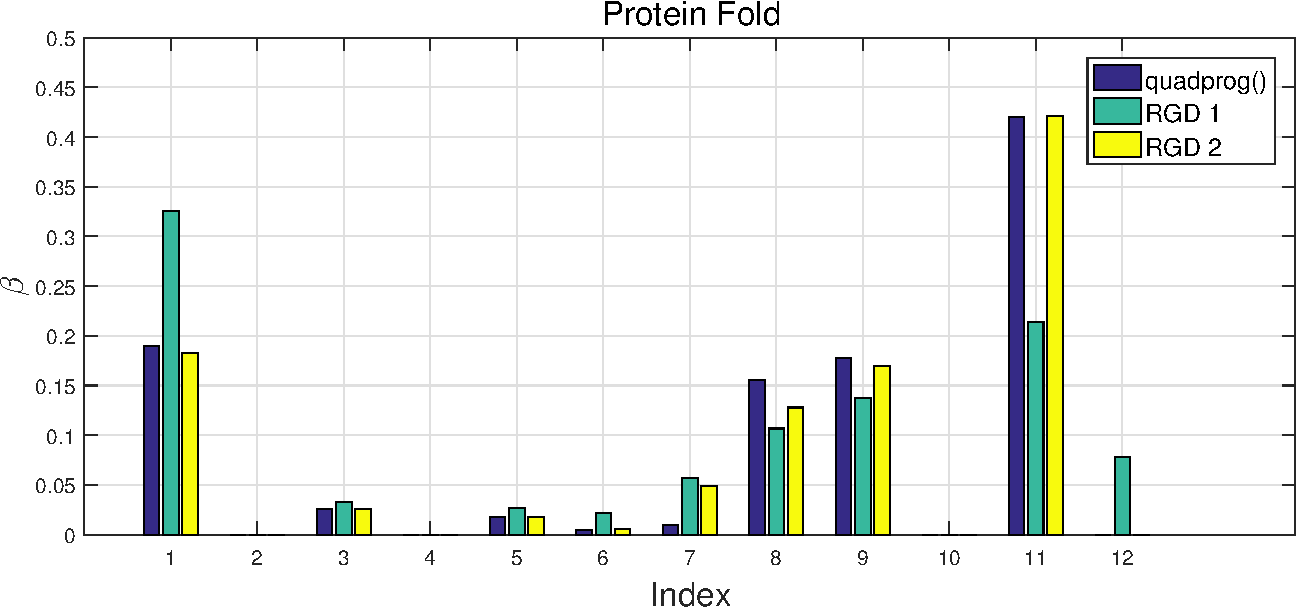
\includegraphics[width=\textwidth]{./fig/comparison_proteinFold-crop.pdf}
\caption{Comparison of $\boldsymbol{\beta}$ obtained from the three optimization processes on \emph{Protein Fold}.}
\label{fig:comparison_beta}
\end{figure*}

\begin{figure*}[t]
\centering
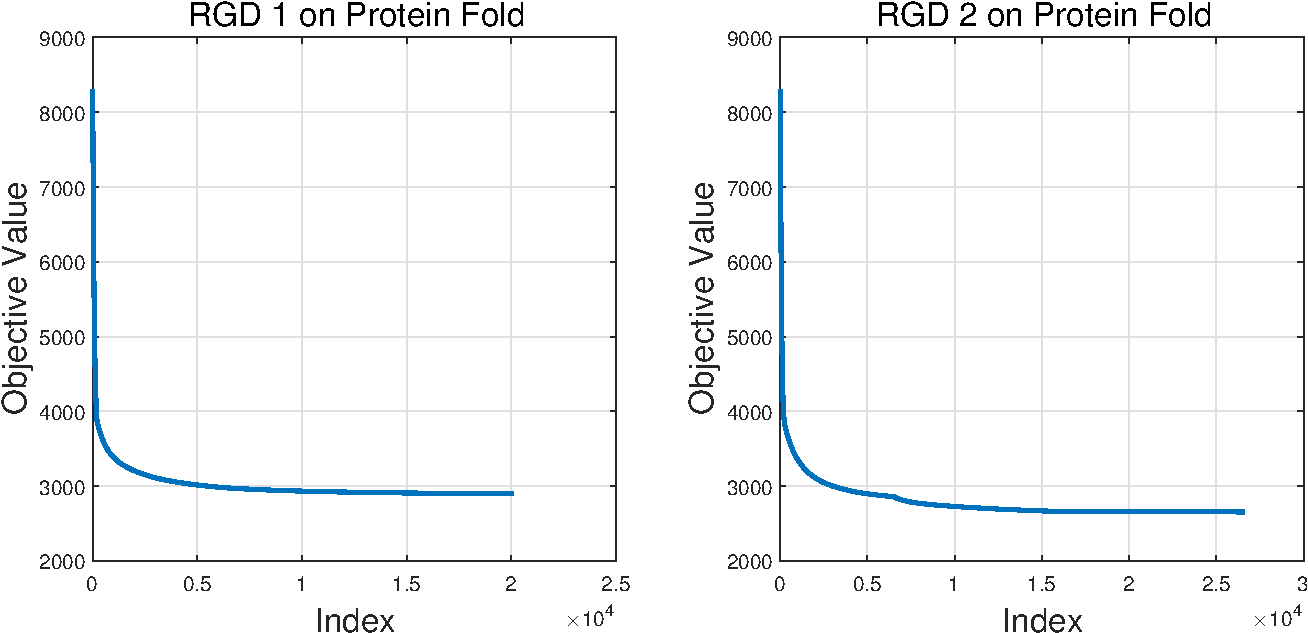
\includegraphics[width=\textwidth]{./fig/obj_proteinFold-crop.pdf}
\caption{Objective values along with iterations on \emph{Protein Fold}.}
\label{fig:objs}
\end{figure*}



%----------------------------------------------------------------------------------------
%	BIBLIOGRAPHY
%----------------------------------------------------------------------------------------

\clearpage

\bibliographystyle{apalike}

\bibliography{ref}

%----------------------------------------------------------------------------------------


\end{document}
